\newpage
\section{NumPy, SciPy, and matplotlib}
\subsection{numpy}
These three libraries form the basis of many (probably most) of scientific Python scripts. NumPy provides a numpy array, a fast way of storing numerical data in memory, and functions to work with them. SciPy provides a large number of algorithms including least squares fitting, signal processing, or spatial clustering and matplotlib allows for the creation of high-quality and customizable plots. Both are designed to work with numpy arrays.

\begin{syntax}[Package installation -- pip]
    Packages that are not installed by default can be installed using a command line utility \ls{pip} which downloads packages registered in the Python Package Index (PyPI, \url{https://pypi.org/}). For example, the install the package \ls{lmfit} run the following command in the command line (also works in the ipython REPL, e.g., in Spyder)
    \begin{lstlisting}
        pip install lmfit
    \end{lstlisting}
    To remove the package use \ls{uninstall}, and to upgrade \ls{install -U}. Run \ls{pip help} for a complete list of available commands. If your virtual environment is activated, pip installs packages in this virtual environment.

    If you are using \ls{uv}, the command \ls{uv pip} is compatible with standard \ls{pip}, e.g., you can use \ls{uv pip install lmfit}. Or, if you want to package your project to be used by other people, you can use \ls{uv add lmfit} which also adds \ls{lmfit} as a requirement of your package.
\end{syntax}

To use numpy we do
\begin{lstlisting}
    import numpy as np
\end{lstlisting}
there are several ways to create an array, e.g.
\begin{lstlisting}[caption=Array creation.]
    #directly from lists
    arr = np.array([1,2,3,4])
    #2D array
    arr_2D = np.array([[1,2,3],
                       [4,5,6],
                       [7,8,9]])
    # similar to list(range()), but none of the start, stop, or step have to be integers
    arr = np.arange(start, stop, step)
    #linearly spaced values
    arr = np.linspace(start, stop, count)
    #filled with zeros
    np.zeros(length)
    #filled with ones
    np.ones(length)
\end{lstlisting}

By default np arrays store type float. For ones and zeros it is often useful to use boolean values (True and False) as \lstinline{np.ones(10, dtype=bool)} will create an array of length 10 filled with True values. Arithmetic works on an element by element basis, therefore when we add/multiply/divide/compare the arrays must be the same length, e.g.,
\begin{lstlisting}
    >>> np.array([1,2,3]) + np.array([4,5,6])
    array([5,6,7])
\end{lstlisting}
However, if one of the operands is a scalar number, the operation \emph{broadcasts}, e.g.,
\begin{lstlisting}
    >>> np.array([1, 2, 3]) + 10
    array([11, 12, 13])
\end{lstlisting}

Array slicing works similarly to list slicing, e.g., \lstinline{arr[start:stop:step]}. Additionally, we can also index into an array using a list of indices, e.g., \lstinline{arr[[0, 2, 4]]} will return an array containing 1st, 3rd and 5th element of array \lstinline{arr}. Finally, using boolean arrays we can create an array subset of elements where the indexing array is true, e.g.,
\begin{lstlisting}
    arr1 = np.linspace(0, 10, 50)
    b = np.sqrt(arr1) > 3 # array of bools True where np.sqrt(arr1) > 3
    arr1[b] # only the elements of arr1 whose square root is larger than 3
\end{lstlisting}

\begin{exercise}
    Write a program that will (in a loop) add numbers $1 + 2 + 3 + ... + n$ for any $n$ using \verb|numpy| arrays and compare it with the Gauss' expression $n(n+1)/2$ for user-supplied $n$. \emph{Hint:} \verb|np.arange|
\end{exercise}
\begin{exercise}
    Write a function, which will return all prime numbers smaller than $N$ using the Sieve of Eratosthenes method. \emph{Hint:} \verb|enumerate()|, \verb|np.ones(N, dtype=bool)|, boolean array masking.
\end{exercise}

\subsubsection{Basic measures and operations with the arrays}
Since numpy arrays are intended primarily for numerical data, there are several methods built into them that calculate some basic measures, e.g.,

\begin{tabular}{lll}
\ls{arr.mean()} & mean of the array\\
\ls{arr.std()} & standard deviation, biased estimate of the variance\\
\ls{arr.sum(), arr.cumsum()} & the sum and cumulative sum\\
\ls{arr.max(), arr.min()} & maximum and minimum, respectively\\
\ls{arr.argmax(), arr.argmin()} & the index of maximum and minimum, respectively\\
\end{tabular}

As for any container type \ls{len(arr)}, returns the length of the array. These also exist in their function forms (e.g., we can call \ls{np.mean(arr)}). Additionally, there are useful functions that deal with arrays in the module itself: \ls{np.diff(arr)} returns an array of differences between nearest neighbors one shorter than \ls{arr}; for more general weighted averaging one can use \ls{np.average(arr, weights)}. Most of these functions have their corresponding nan- versions, which ignore NaN values in the arrays (e.g., \ls{np.nansum, np.nanmax} etc.). \ls{np.isnan(arr)} returns an array of the same length as \ls{arr} with True everywhere where \ls{arr} was NaN. For boolean-valued arrays the extension of \ls{and} and \ls{or} are \ls{np.logical_and(arr1, arr2)} and \ls{np.logical_or(arr1, arr2)} and similarly \ls{np.logical_not(arr)}, which create a new array with the logical operation applied to every element of the input arrays. Logical operators by themselves do not work with arrays.

\begin{syntax}[NaNs and Infs.]
     Mathematical operations can result in either a Not-a-Number (NaN) or infinities, which are represented in numpy by \ls{np.nan} and \ls{np.inf}. These are special values indicating, for NaN, that an undefined operation was performed, e.g., \ls{np.log(-1)} (Python and Numpy support complex numbers, but operations with real numbers are assumed to result in reals as well -- if we wanted to use the complex logarithm we would have to give it a complex -1, i.e., \ls{np.log(-1 + 0j)}).

    Simple division by zero, e.g., 1/0, will result in a ZeroDivisionError error. However, when part of an \ls{np.array} it will result in an $\pm$np.inf and a Warning, e.g., try running \ls{np.array(1)/np.array(0)}.

    The idea of not crashing on undefined operations or division by zero is in the idea that often only part of the array is damaged (e.g., a -1 can be a placeholder for a value that's not available) and it might be easier and cleaner to proceed assuming that all operations are valid and then simply throw out the NaNs at the end.
\end{syntax}

An array can be sorted in-place using \ls{arr.sort()} or a new sorted array can be created using \ls{sorted_arr = np.sort(arr)}. To get an array of indices that would sort the array we can use \ls{np.argsort()}, which is useful when we want to sort one array according to another, e.g.,
\begin{lstlisting}
    import numpy as np
    items = np.array(["Eggs", "Bread", "Apples"])
    prices = np.array([50, 20, 40])

    sort_ix = np.argsort(prices)
    print("Items sorted according to prices:")
    print(items[sort_ix])
\end{lstlisting}

\subsubsection{File I/O}
We will be using numpy and matplotlib to analyze some experimental data. First, we need to get the data, typically from some file on the disk. Assuming that we have data stored as a text file in \verb|data.txt| as two columns of numbers separated by tabs we can load it into a 2D numpy array using
\begin{lstlisting}
    arr = np.loadtxt("data.txt", comments='%', skiplines=3)
\end{lstlisting}
which loads \verb|data.txt| into 2D array \verb|arr|, ignores all lines beginning with \% and skips first three datalines. If, rather than tabs our data is separated by commas (i.e., a \verb|.csv| file) we can add a keyword argument \verb|delimiter=','| or use \lstinline{np.loadcsv()}.

\begin{syntax}[Paths]
    Paths to files or directories can be absolute or relative. Absolute path specifies the absolute position of a file in the filesystem, on Windows it will typically begin with something like \verb|C:\| and on Linux or Mac with the root directory \verb|/|.

    A relative path is relative to the current working directory, which can be obtained using \ls{getcwd()} from the \ls{os} module.

    Different operating systems use different directory separators, i.e., Windows uses \verb|\|, Linux and Mac \verb|/| and Japanese Windows computers use \verb|¥|. To join directory names in a way that will work everywhere we can use \ls{os.path.join('dir1', 'dir2', 'dir3', ...)}.

    To find multiple files whose name fit a pattern we can use the function \ls{glob()} from the module \ls{glob()}. For example, \ls{glob(os.path.join("photos", "photo*.png"))} will return a list of all files that fit the pattern \ls{"photos/photo<any number of any characters>.png")}
\end{syntax}

Using the file I/O functions from Python standard library is also possible. The function \lstinline{file = open(filename, mode)} opens the file in a given mode, most common are \lstinline{'r'} for reading, \lstinline{'w'} for (over)writing, and \lstinline{'a'} for appending. All contents of the file can be read in one go using \lstinline{file.readlines()} or we can iterate over the lines of the file using a for loop (see example below). Inversely, there is \lstinline{file.write(some_string)} (if the file is opened with mode 'r' this will fail). Especially for writing, it is important to call \lstinline{file.close()} after we are done with the file otherwise the changes might not be written to the disk due to caching.

The \lstinline{np.loadtxt()} with default arguments is roughly equivalent to
\begin{lstlisting}
    import numpy as np
    def my_load(fn):
        with open(fn, 'r') as file:
            rows = []
            for line in file:
                row = [float(s) for s in line.strip().split()]
                rows.append(row)
        return np.array(rows)
\end{lstlisting}
\begin{syntax}[with statement (basic)]
\lstinline{with} is an example of so-called context management which ensures that resources (in this case a file) are properly cleaned up after we are done using them. We will learn how to create our own context managers later, for now, the code
\begin{lstlisting}
    with open(fn, 'r') as file:
        do_stuff()
\end{lstlisting}
    is roughly equivalent to
\begin{lstlisting}
    file = open(fn, 'r')
    do_stuff()
    file.close()
\end{lstlisting}
with the caveat that \ls{with} ensures that \lstinline{file.close()} runs even if \lstinline{do_stuff()} crashes the program.
\end{syntax}

\begin{exercise}
    Extend the \lstinline{my_load(fn)} from the example above to support comments in the files.
\end{exercise}

\subsection{matplotlib}

matplotlib allows plotting data. We plot data inside axes, which are contained in figures. A figure can contain multiple axes. The simplest way to create a new figure with new axes is \footnote{Note that \lstinline{plt.subplots()} returns two values. It only returns a single tuple, which is desctructured, or unpacked, into two variables \lstinline{fig} and \lstinline{ax}.}
\begin{lstlisting}
    import matplotlib.pyplot as plt
    fig, ax = plt.subplots()
\end{lstlisting}
If we have data in arrays \lstinline{x} and \lstinline{y} of the same length we can plot them using, e.g., 
\begin{lstlisting}[caption=Basic plotting.]
    ax.plot(x, y, '-') # connect the pairs of points given by x and y with full lines
    ax.semilogy(x, y, '--s') # logarithmic y-axis, dashed line with square markers
    ax.loglog(x, y, ':') # logarithmic x and y axis, dotted line
    ax.scatter(x, y) #scatter plot, does not connect the points by lines
\end{lstlisting}
The plotting format is specified using a format string immediately following the data which has the format \ls{fmt = [marker][line][color]}.\footnote{See \url{https://matplotlib.org/stable/api/_as_gen/matplotlib.pyplot.plot.html} for complete list of possible formats} We can specify the line width using \ls{lw=} keyword, marker size using \ls{ms=} and color using \ls{color=} \footnote{See \url{https://matplotlib.org/stable/users/explain/colors/colors.html}} Note that matplotlib does not care whether the pair of arrays x and y represents a mathematical function, it will simply connect the points sequentially with lines.

To label the axes we can use \ls{ax.set_xlabel()} and \ls{ax.set_ylabel()}. Data can be labeled by passing \ls{label=} keword argument with a string to any of the plotting commands and then calling \ls{ax.legend()}. We can save the figure using \ls{fig.savefig(filename)}.

For example, to plot a Gaussian with magenta lines and cyan points we can do
\begin{lstlisting}[caption=Complete plotting example.]
import numpy as np
import matplotlib.pyplot as plt

xs = np.linspace(0, 10, 100)
ys = np.exp(-(xs - 5)**2)

plt.close('all') #closes all figures we have opened so far
fig, ax = plt.subplots()

ax.plot(xs, ys, '--s', ms=5, lw=2, color='magenta', label=r'ax.plot($e^{-x^2}$)')
ax.scatter(xs, ys, s=ys*10, marker='o', color='cyan', zorder=3,
           label=r'ax.scatter($e^{-x^2}$)')

ax.set_xlabel('$x$ values')
ax.set_ylabel(r'the gaussian $e^{-(x-5)^2}$')
#where to put the legend, we can also use "best" and let matplotlib guess
ax.legend(loc='upper left')

fig.tight_layout() #reduces some of the whitespace around edges
fig.savefig('gaussian.pdf') #the file format of the image is deduced from the extension
\end{lstlisting}
\begin{center}
    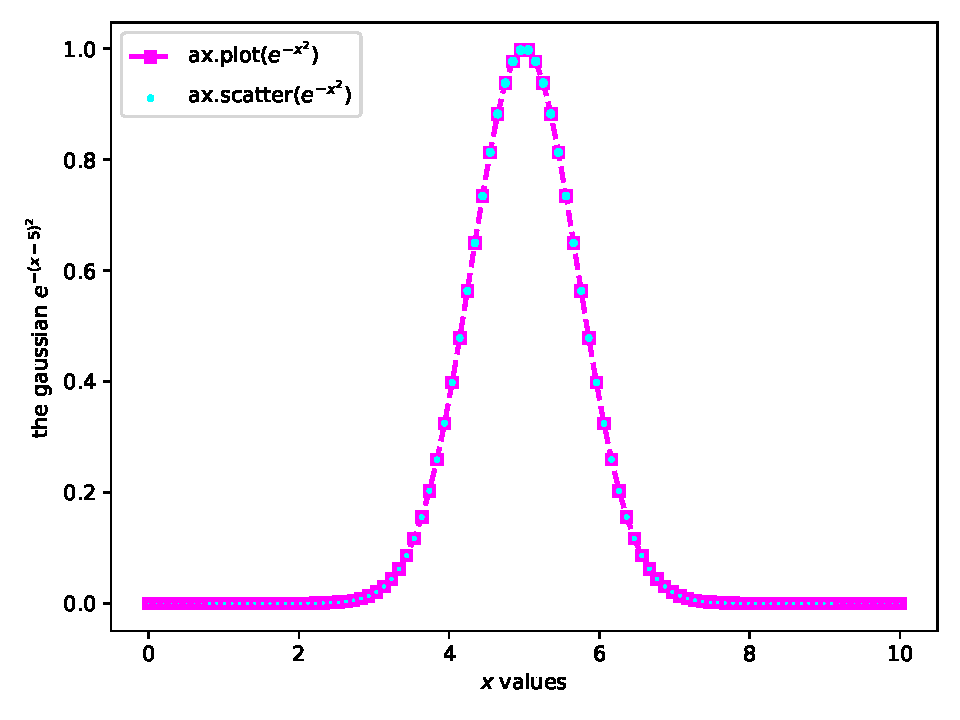
\includegraphics[width=0.5\linewidth]{gaussian.pdf}
\end{center}
Notice that we can control which objects are drawn on top of which using the \ls{zorder=} keyword argument and that basic \LaTeX math typesetting is supported, but latex commands beginning with backslash need to be either escaped (i.e., \verb|"$\\frac{}{}$"|) or in raw strings (i.e., \verb|r"$\frac{}{}$"|).

\begin{exercise}
    Write a program, which will, using NumPy and Matplotlib, graph the expressions $y=x$, $y=x^2$ and $y=\sqrt{x}$ from $x=0$ to $x=5$ with different line styles (e.g., full line, dashed, dotted) and user-supplied number of points. Try linear, semilogarithmic and logarithmic axes. Label the axes and the curves.
\end{exercise}

One figure can contain multiple axes created by passing the optional rows and columns arguments to \ls{plt.subplots()}. The multiple axes are created in a regular grid with a specified number of rows and columns. For axes of unequal sizes, we can specify ratios of their widths and heights using \ls{width_ratios} and \ls{height_ratios} (see \ls{gridspec} \footnote{\url{https://matplotlib.org/3.5.0/tutorials/intermediate/gridspec.html}} for more complicated figure layouts). The axes can share the x and y ranges by specifying the boolean keyword arguments \ls{sharex} and \ls{sharey}, respectively, for example
\lstinputlisting[caption=Multiple axes in single figure.]{../example_code/multiple_axes.py}
\begin{center}
    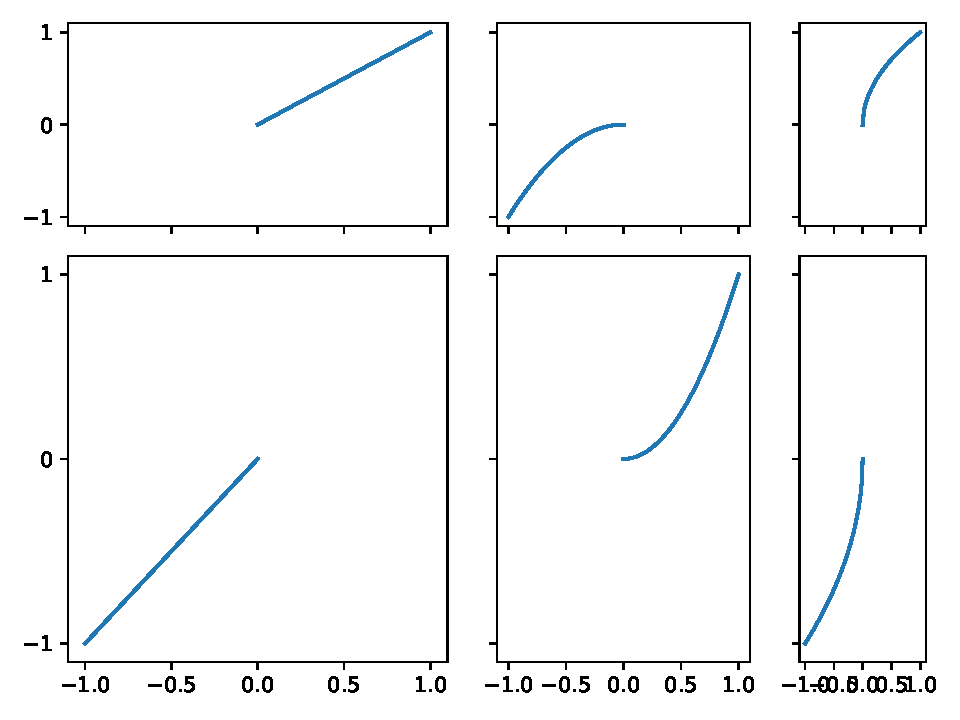
\includegraphics[width=0.5\linewidth]{multiax.pdf}
\end{center}
\begin{exercise}
    \label{ex:peak}
    Write a program that will read the data from "data.txt" which contains three columns of numbers separated by tabs. Let's call these columns frequency, $X$ and $Y$. Plot the frequency dependence of $X$ and $Y$ 
    \begin{enumerate}
        \item in the same axes ($X$ full line, $Y$ dashed line)
        \item in separate axes in the same figure sharing x and y range
    \end{enumerate}
    Plot also $X$ vs. $Y$ in a seprate plot. Label the axes appropriately.
\end{exercise}
\begin{syntax}[Writing modules.]
    Any python file can be imported by any other python file as a module using the \ls{import} keyword, the name of the module is the name of the file (without the .py ending). When \ls{import}ed, the file is first executed, i.e., any code that sits outside of function definitions will run, for example, take two files in the same directory

    \verb|module.py|:
    \begin{lstlisting}
        def my_module_function(x):
            return 1 + x

        print("Hello modules!")
    \end{lstlisting}

    \verb|module_user.py|:
    \begin{lstlisting}
        import module as m
        print(m.my_module_function(1))
    \end{lstlisting}

    Upon running \verb|module_user.py|, "Hello modules!" will be printed. This is usually not desirable. To prevent any code from running when imported and only allow it to run when the file is run directly we can do
\begin{lstlisting}
    if __name__ == '__main__':
        print("Hello modules.")
\end{lstlisting}
    Here, \ls{__name__} is a special variable defined by Python itself that contains the name of the module associated with the current file. Its value is \ls{'__main__'} if and only if it was directly.

    To import a file as a module Python must be able to find it. By default, Python looks in the current working directory \ls{os.getcwd()} and in the directories listed in the list \ls{sys.path} in the package \ls{sys}. If we want to load a package from somewhere else we can simply \ls{sys.path.append()} its directory to the path variable.
\end{syntax}
\begin{exercise}
    \label{ex:peaks}
    Find the maximum and the minimum of the absolute value $R = \sqrt{X^2 + Y^2}$, and indicate their positions using vertical lines in the graph of frequency dependence of $X$ and $Y$ from the previous exercise. Estimate the full-width-at-half-maximum (FWHM) of the peak and the quality factor $f_0$/FWHM, where $f_0$ is the frequency of the maximum response. 
    
    \emph{Hint:} \ls{np.argmin, np.argmax}, \ls{ax.axvline, ax.axhline}
\end{exercise}
\begin{exercise}
    \label{ex:peaks-all}
    Process all files from \ls{lots_of_data} directory similarly to Exc.~\ref{ex:peaks}. Plot the FWHM as a function of $f_0$. Use the solution to Exc.~\ref{ex:peaks} as a module.
    
    \emph{Hint:} \ls{glob}
\end{exercise}

Observables that depend on two control variables can be often plotted using heat maps, for which we can use \ls{ax.imshow(arr2D)}, which takes a 2D array of numbers and maps them to a color of a pixel using a colormap\footnote{See \url{https://matplotlib.org/stable/users/explain/colors/colormaps.html} for a full list of colormap names.} Note however, that \ls{imshow()} is primarily used for images, which conventionally start in the upper left corner with left-handed axes. Data typically start in the lower-left corner with right-handed axes. This can be changed changed by specifying \ls{origin='lower'} keyword to \ls{imshow()}. Alternatively, for plotting data which are not on a regular grid we can use \ls{ax.pcolormesh(X, Y, Z)} where \ls{X, Y, Z} are 2D arrays.

For example, to plot a 2D Gaussian with the \ls{'inferno_r'} colormap,
\begin{lstlisting}[caption=Two-dimensional plotting example.]
import numpy as np
import matplotlib.pyplot as plt

#x and y axis
_xs = np.linspace(0, 10, 100)
_ys = np.linspace(0, 10, 100)
#but we need 100 x 100 points for both x and y that sample the 
#the entire interval (0, 10) x (0, 10), this can be done using
#meshgrid
xs, ys = np.meshgrid(_xs, _ys)
zs = np.exp(-(xs - 5)**2 - (ys - 5)**2)

plt.close('all') #closes all figures we have opened so far
fig, ax = plt.subplots()

plot = ax.imshow(zs, cmap='inferno_r', origin='lower')
#similar
#plot = ax.pcolormesh(xs, ys, zs, cmap='inferno_r') 
cbar = fig.colorbar(plot) #the color axis scaling
cbar.set_label('$z$')
ax.set_xlabel('$x$')
ax.set_ylabel('$y$')
\end{lstlisting}
\begin{center}
    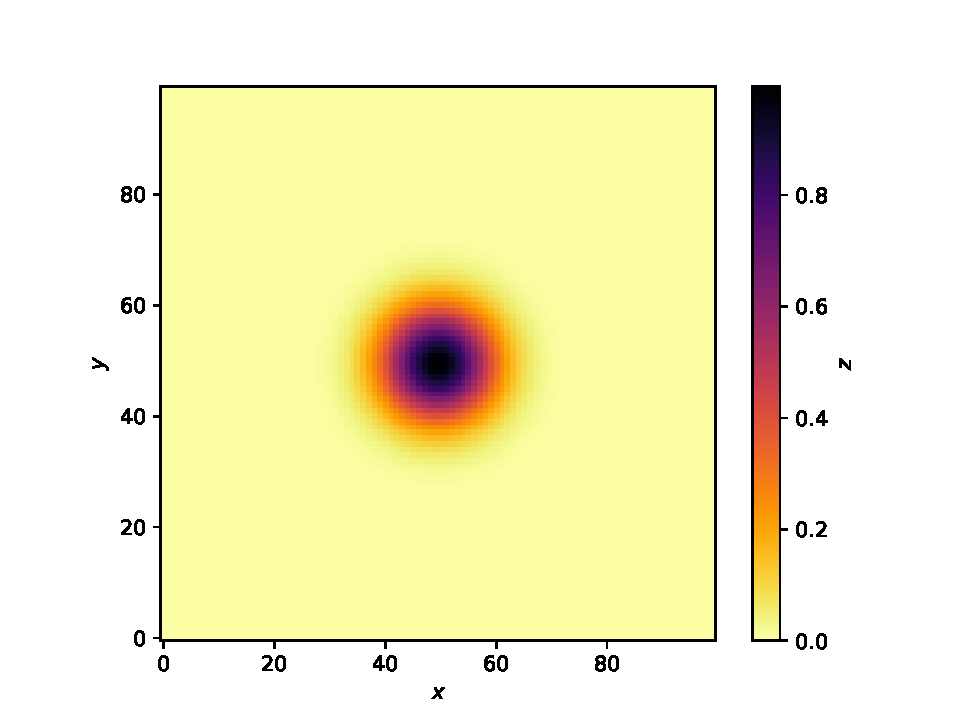
\includegraphics[width=0.5\linewidth]{gaussian_2D.pdf}
\end{center}
\begin{exercise}
    Plot the Mandelbrot set with configurable range and resolution.

    \emph{Hint:} The Mandelbrot set is a set of complex numbers $c$ for which the series $z_{n+1} = z_n^2 + c,\; z_0 = 0$ does not diverge. If $z_n \geq 2$ for any $n$ the series will diverge. As a convergence criterium we can use that $z_n < 2\; \forall n < N_\mathrm{max}$ ($N_\mathrm{max} = 100$, for example). Plot the set using \ls{plt.imshow(c)} where \ls{c[i,j]} is the number of interactions needed to exceed $z_n = 2$ (or $N_\mathrm{max}$). The entire set is contained in the rectangle with lower-left corner $-2-i$ and upper-right corner $1+i$ in the complex plane.
\end{exercise}

\subsubsection{Review of basic plotting commands}
Assuming that the figure and axes were created as \ls{fig, ax = plt.subplots()}, the basic commands for manipulating the plot are

\begin{tabular}{p{40mm}p{100mm}}
     \ls{ax.xlabel("the x-label"), ax.ylabel("the y-label")} & sets the axis labels \\
     \ls{ax.set_xlim(xmin, xmax), ax.set_ylim(ymin, ymax)} & sets the axes limits, xmin, xmax etc. can also be used as keywords \\
     \ls{ax.set_aspect('equal')} & sets the aspect ratio of the axes to be equal, useful when both axes contain qualitatively similar data\\
     \ls{ax.legend(loc=location)} & shows the legend at locatoin \ls{location} $\in$ \ls{"upper|lower left|right"} or \ls{"best"} \\
     \ls{fig.tight_layout()} & adjust the axes size to fit all labels and reduces whitespace\\
     \ls{fig.supxlabel('xlabel'), fig.supylabel('ylabel')} & sets the common figure-wide axis labels for multi-axis figures\\
     \ls{fig.colorbar()} & creates a colorbar in the figure\\
     \ls{plt.close('all')} & closes all open figures
\end{tabular}